\section{Analisi del Problema}
\labelsec{ProblemAnalysis}
%===========================================================================

\paragraph{Assunzioni}
Prima di iniziare l'analisi del problema abbiamo ritenuto neccessario effettuare delle assuzioni riguardanti al paradigma che ci consentirebbero di effettuare un prodotto di qualit\`a migliore e con meno sforzi.

Il paradigma di programmazione di riferimento \`e il \textit{reactive programming} perch\'e la concezione di flusso di dati \`e proprio quello che ci interessa modellare in quanto anche nel nostro sistema sar\`a presente un flusso di dati dal client al server. Per la comunicazione attraverso la rete questo ci consente di sfruttare chiamate asincrore aumentando il disaccoppiamento tra client e server.

Per questo abbiamo deciso di utilizzare per i dati un database NoSQL per via dell'estrema dinamicit\`a, in quanto ci consente di aggiungere dei campi anche in seguito e un miglioramento di performance nell'accesso a dati che normalmente richiederebbero dei join.

Per ulteriori informazioni pi\`u dettagliate sul paradigma si rimanda ad un'altra sede. 

\subsection{Architettura Logica}

Per la costruzione dell'architettura logica ci si baser\`a ovviamente sulla precedente analisi dei requisiti in modo da mantenere il contatto con questi e non rischiare di uscire fuori specifica. Anche in questo caso si andr\`a separare l'analisi in due parti:

\begin{itemize}
\item Sistema Embedded
\item Server e Website
\end{itemize}

La parte del website \`e stata incorporata direttamente nella parte server proprio per la sua assenza di business logic.

\paragraph{Modellazione Reactive}

Prima di iniziare a costruire la modellazione sulla base del paradigma appena citato \`e necessario capire come fare a modellare lo stream stesso all'interno della nostra architettura logica, conseguentemente si \`e deciso di utilizzare i \textit{marable diagrams}. Questi sono una rappresentazione di come il flusso di dati nel tempo avviene e quali tipologie di trasformazioni consentono di effettuare.

Con questi schemi ci viene concesso ancora una volta di concentrarci prima sul ''cosa'' e non sul ''come'' che invece viene delegata alla parte progettuale, dove si cercher\`a effettivamnete di implementare il risultato finale dell'analisi

\subsubsection{Sistema Embedded}

\begin{center}
  \textbf{Flussi Dati}
\end{center}

Alla luce del paradigma di programmazione che si \`e deciso di adottare sono stati effettuati dei cambiamenti anche alla struttura che \`e stata esposta precedentemente proprio perch\'e ci sono state fornite da questa assunzione nuovi livelli di astrazione, primo tra tutti il concetto di \textbf{Stream/Flusso}. Quindi in questa fase abbiamo ritenuto molto utile iniziare a visualizzare effettivamente questi flussi tramite un'apposito diagramma.

% Figura fatta con draw.io
\begin{figure}[ht]
\centering
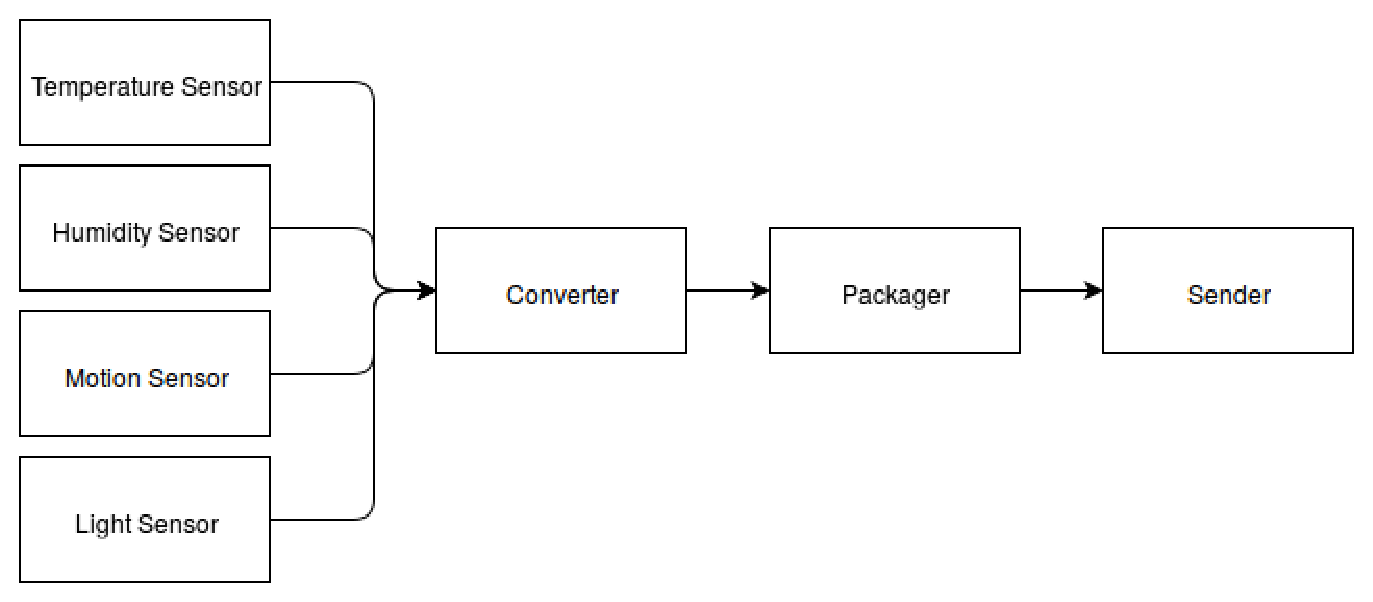
\includegraphics[width=\textwidth]{Figures/LogicArchitecture/EmbeddedSystem/FlowDiagram}
\caption{Diagramma di flusso, per sensore, dei dati}
\end{figure}


In particolare si puo' notare come in questo diagramma il compito di convertire i valori di un sensore sia stato disaccoppiato dal sensore stesso che quindi si deve solamente occupare di invitare i dati all'interno del flusso. \`E stato inoltre aggiunto anche una nuova entit\`a \textit{packager} che si occuper\`a di formattare i valori secondo il protocollo che deve essere definito tra client e server per l'apposita comunicazione. In particolare ogni dato proveniente da un sensore avr\`a un suo formato per via: della differenziazione dei dati, della tempistica di rilevazione che pu\`o anche risultare diversa e dell'idea percui la comunicazione in ogni caso debba essere asincrona.

Sulla base di questa ultima frase si vuole sottolineare che ogni sensore quindi avr\`a un suo flusso asincrono, ma che in quest'immagine si \`e deciso di condensare in un'unica immagine per comodit\`a.

Di seguito si indica un primo marable diagram che mostra le varie trasformazioni che verranno applicate. Questo serve soprattutto per iniziare a capire poi come interpretare eventuali altri schemi come questo.

% Figura fatta con draw.io
\begin{figure}[ht]
\centering
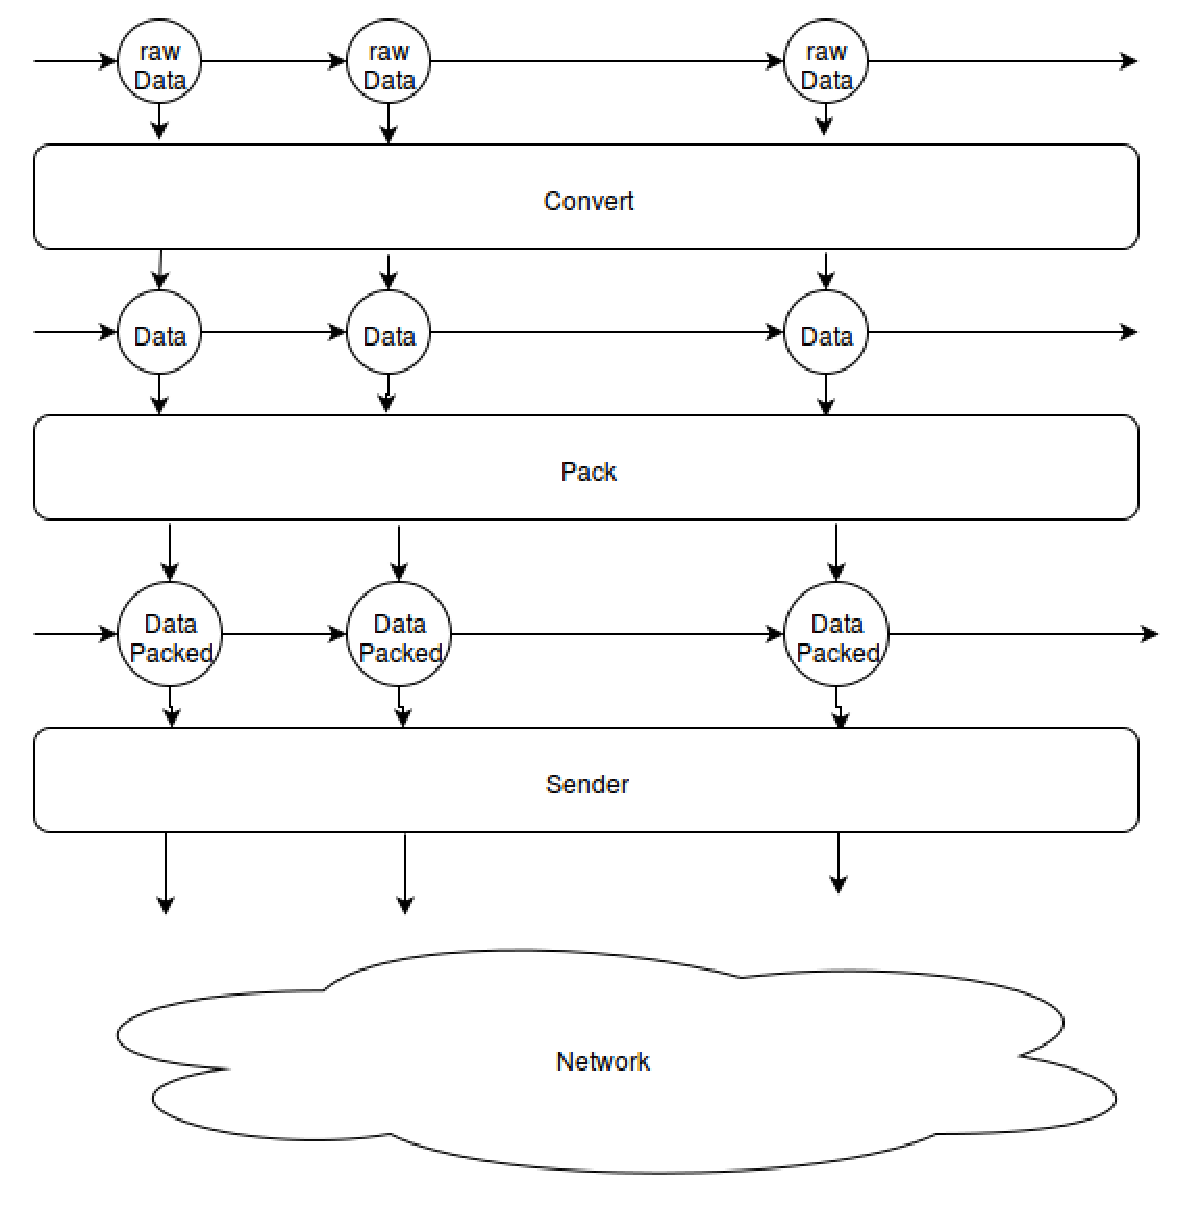
\includegraphics[scale=0.7]{Figures/LogicArchitecture/EmbeddedSystem/MarableDiagram}
\caption{Marable diagram dei singoli dati proveniente da una sorgente}
\end{figure}


\afterpage{\clearpage}

\newpage

\begin{center}
  \textbf{Struttura}
\end{center}

Chiaramente la struttura, che si basa sul precedente step di analisi dei requisiti, risulta cambiata anche alla luce delle assunzioni effettuate e quindi si possono notare l'introduzione di alcune entit\`a che servono per la gestione del sistema embedded e per impostare i flussi di dati provenienti dai sensori.

\begin{figure}[h]
\centering
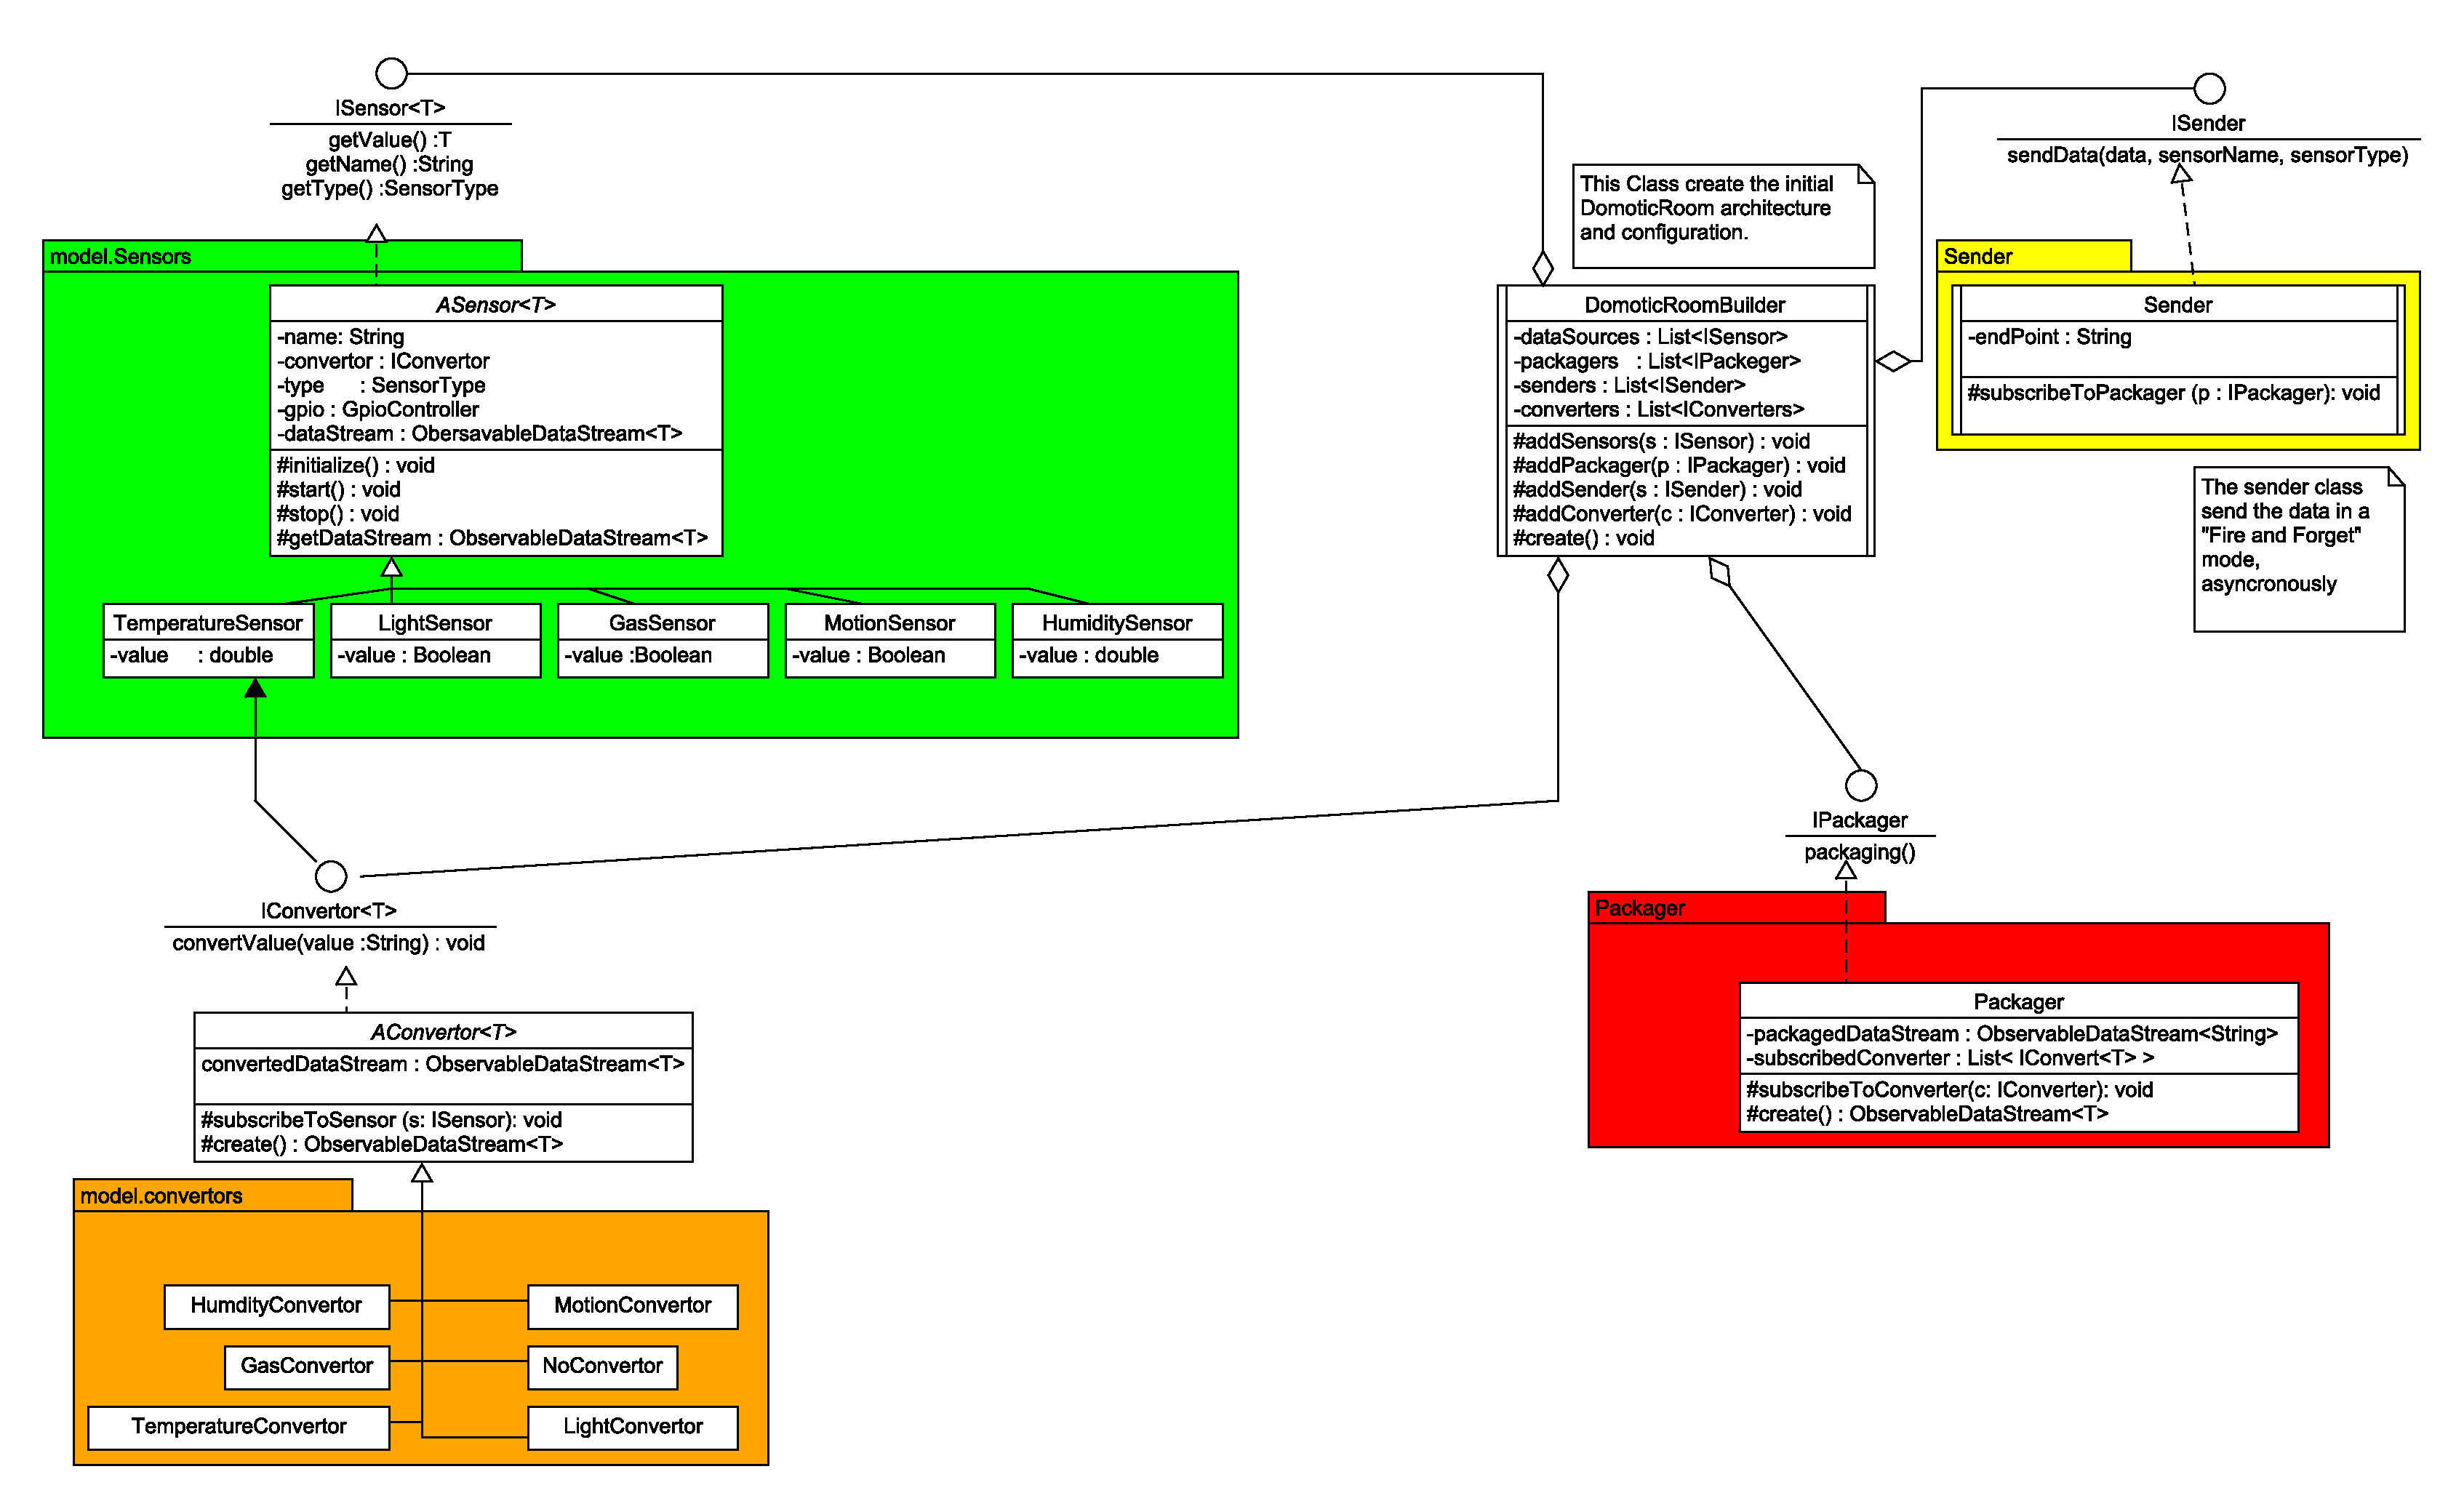
\includegraphics[scale=0.2]{Figures/LogicArchitecture/EmbeddedSystem/Structure}
\caption{Logic Architecture, Structure}
\end{figure}

Come si mostra nello schema soprastante, la struttura logica non ne esce particolarmente modificata rispetto all'analisi iniziale.\\
Il \textit{SensorDataFetcher} è stato eliminato, poich\`e l'implementazione di polling per ricevere dati dai sensori viene sostituita dal pattern Observable, utilizzato per sfruttare tutte le potenzialità del paradigma Reactive. \\
La nuova entit\`a \textit{DomoticRoomBuilder} ha il ruolo centrale di inizializzare il sistema, creando l'architettura e la configurazione iniziale dei suoi componenti.\\
L'entit\`a \textit{Sensor} ha il ruolo centrale di ricevere i dati dai sensori e inviarli su uno stream dati osservabile.
L'entit\`a \textit{Convertor} si occupa di convertire i dati che riceve dalla sorgente \textbf{Sensor} a cui è sottoscritto; inoltre genera un nuovo Stream dove invia i dati convertiti che riceve dai \textit{Sensor} a cui è sottoscritto.\\
L'entit\`a \textit{Packager} unisce tutti i flussi in entrata, dai \textit{Converter} in un unico flusso, il suo compito è preparare i dati ad essere inviati al Server.\\
L'entit\`a \textit{Sender} si occupa di inviare i dati che riceve dal Packager sulla rete, come pensato nella struttura iniziale.

\begin{center}
  \textbf{Interazione}
\end{center}

La parte di interazione viene drasticamente modificata proprio perch\'e l'assunzione del paradigma reactive risulta principalmente improntato su questo, in particolare \`e possibile condensare in meno codice, e pi\`u dichiarativo. Vengono in ogni caso mostrati le varie operazioni effettuate sullo stream per mantenere il contatto con quanto mostrato attraverso i marable diagrams. Particolare attenzione va posta poi sulla parte che converte da \textit{procedure calls} a \textit{reactive streams}. \\
Il sistema non ha una interazione continua; come invece suggerisce il paradigma, esso "reagisce" al verificarsi di un evento di particolare interesse.\\
In questo caso, il sistema reagisce autonomamente alla ricezione di un valore inviato dal sensore. L'entit\`a \textit{Sensor} si occupa di incanalare queste letture periodiche in un flusso potenzialmente infinito di valori.\\
L'entit\`a \textit{Convertor} \`e a sua volta interessata all'arrivo di un nuovo valore sul flusso creato dal \textit{Sensor}; il Convertor applicher\`a ad ogni nuovo dato una funzione atta a convertire in valore in un dato di maggiore utilità per il sistema.\\
L'entit\`a \textit{Packager} sarà invece di ascolto sui flussi generati da ogni \textit{Convertor}, appena un nuovo valore convertito è inviato sul flusso; a questo punto il suo compito \`e "impacchettare" il dato, secondo un protocollo di trasmissione per poterlo inviare al Server.\\
Quest'ultima parte \`e gestita dal \textit{Sender} che appena un dato impacchettato \`e pronto lo invier\`a al Server.\\
L'iterazione delle entit\`a del server \`e ben rappresentata dal diagramma di flusso precedentemente esposto.

\begin{center}
\textbf{Comportamento}
\end{center}

Il comportamento atteso dall'Embedded System \`e molto semplice: una entità DomoticRoomBuilder tramite la funzione addSensor() viene creata l'architettura di iterazione sono esposta, terminata l'operazione \`e possibile iniziare la fase di monitoraggio che prevede la lettura dei dati proveniente dai sensori.
 
\begin{figure}[H]
\centering
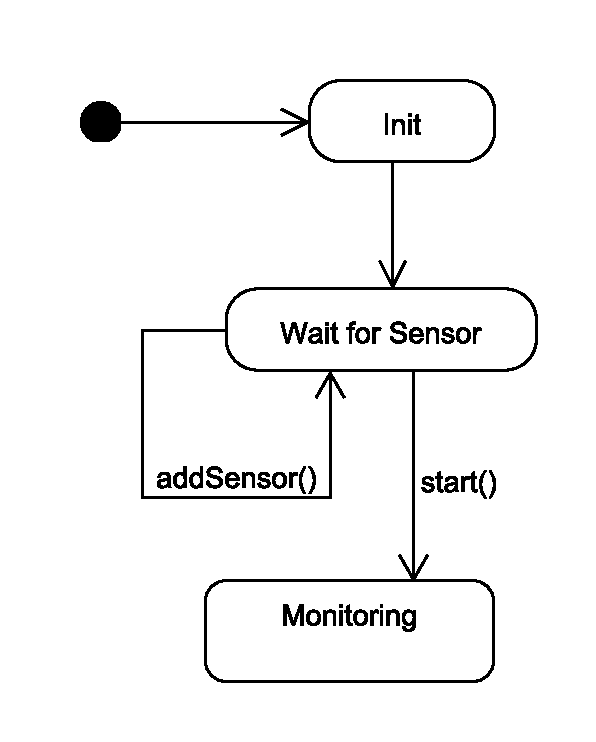
\includegraphics[width=0.5\textwidth]{Figures/LogicArchitecture/EmbeddedSystem/Behaviour}
\caption{Diagramma di comportamento}
\end{figure}

\subsubsection{Server}

\begin{center}
  \textbf{Interazione e Flussi Dati}
\end{center}

Anche per quanto riguarda la parte server \`e necessario definire gli steam che saranno presenti all'interno del sistema. Inquanto questa parte \`e notevolmente pi\`u corposa rispetto a quella dell'embedded system per varie ragioni, prima tra tutte la capacit\`a di calcolo, saranno necessari pi\`u stream, in particolare si \`e pensato di creare uno stream per ogni funzionalit\`a sulla base delle operazioni che quindi sono da compiere.

Il primo flusso che andremo ad analizzare riguarda la ricezione dei dati da parte del sistema embedded. In particolare si vuole cercare di riutilizzare le entit\`a che si sono introdotte nell'analisi dei requisiti proprio perch\'e queste sono maggiormente collegate al dominio. Si pu\`o inoltre notare altre entit\`a chiamate \textit{IRawDataFormatter e IDBDataFormatter}, queste entit\`a sono utili per preparare la corretta formattazione dei dati e la loro validazione, provenienti dal flusso e dalla successiva elaborazione per essere salvati poi sul database. Si \`e deciso in particolare di inserirlo per andare a separare i compiti il pi\`u possibile e per facilitare la modifica nel caso si voglia adottare uno standard dei dati interno rispetto a quello del client in modo da effettuare una netta indipendenza tra server e client. Soprattutto perch\'e in un'eventuale futuro si pu\`o facilmente immaginare un'eterogeneit\`a dei dati dovuti ai vari client disponibili e dalla loro provenienza (altre aziende, protocolli proprietari \ldots)

\begin{figure}[h]
\centering
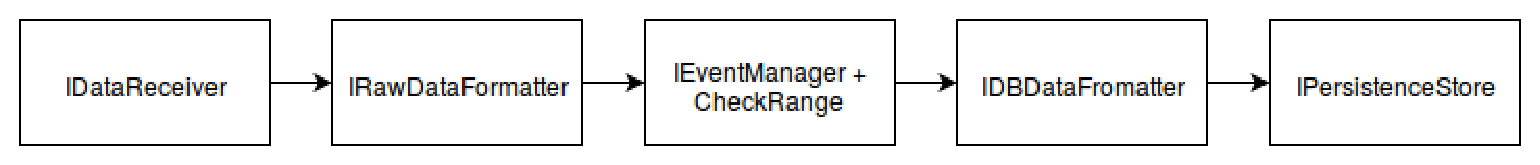
\includegraphics[width=\textwidth]{Figures/LogicArchitecture/Server/FlowDiagramReceiveData}
\caption{Server, Flusso Dati Ricezione}
\end{figure}

Il secondo e ultimo flusso di dati che verr\`a trattato riguardano le richieste di dati stessi per la visualizzazione da parte dell'utente. Probabilmente per quanto riguarda le seguenti operazioni si poteva anche pensare di gestire il tutto attraverso delle semplici chiamate a procedura, ma, per mantenere una certa coerenza, per sfruttare la dichiarativit\`a del paradigma reactive e per evitare di incorrere nel problema noto come \textit{Callback Hell} si \`e scelto di utilizzare comunque un flusso. Un'ulteriore vantaggio di gestire attraverso l'infrastruttura reactive consiste nella possibilit\`a di aggiornare realtime l'interfaccia ogni qualvolta avviene l'inserimento di un nuovo valore. Concludendo si vuole far notare la presenza di un'entit\`a che entra in campo quando viene richiesta un'analisi sui dati e non semplicemente una sua visualizzazione. La forma a nuvola indica proprio la possibilit\`a che questo oggetto entri a far parte o meno nel flusso.

\begin{figure}[h]
\centering
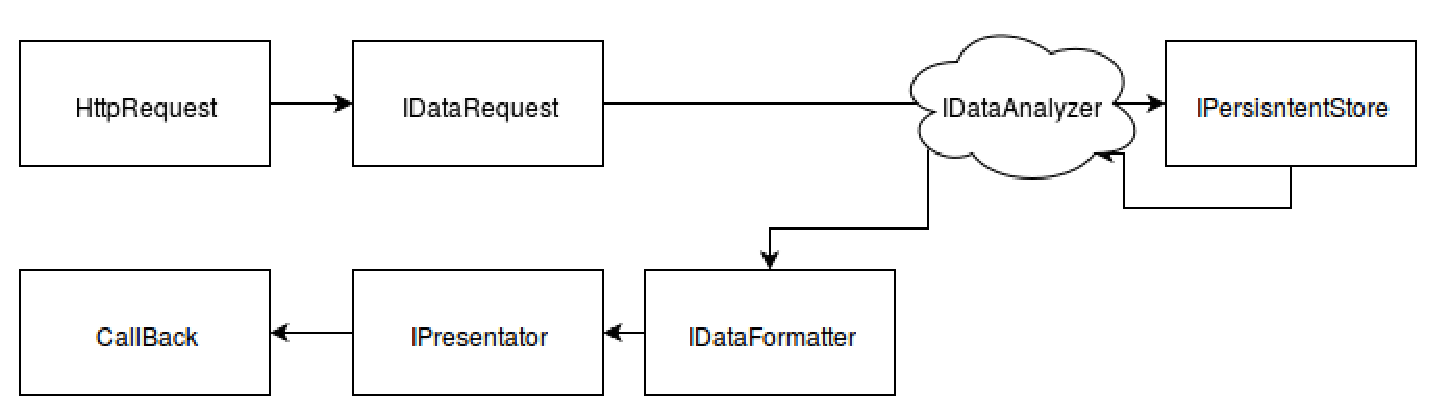
\includegraphics[width=\textwidth]{Figures/LogicArchitecture/Server/FlowDiagramViewData}
\caption{Server, Flusso Dati Richieste Dati}
\end{figure}

\begin{center}
  \textbf{Restanti Interazioni}
\end{center}

Per quanto riguarda  riguarda l'aggiornamento del range da parte dell'utente, in particolare anche in questo caso l'IEventManager viene chiamato in causa il quale si occuper\`a di notificare il cambiamento sia a livello di database che al componente incaricato di controllare il range. Questa parte non subisce particolari cambiamenti rispetto a quella dell'analisi dei requisiti perch\'e rimane molto coerente anche a fronte del cambio di paradigma. Un cambiamento significativo riguarda il fatto che il cambiamento del range non avviene pi\`u direttamente dall'event manager ma dal database, questo per enfatizzare che il cambiamento del range non \`e effettivo se non viene prima registrato in maniera permanente.

Questa interazione non avviene attraverso uno stream ma viene gestito come una chiamata classica http in quanto non richiede che ci sia un dialogo continuo tra le varie parti, client e server. Si riporta in ogni caso sotto forma di flusso di chiamate, quelle che vengono effettuate dall'applicativo.

\begin{figure}[h]
\centering
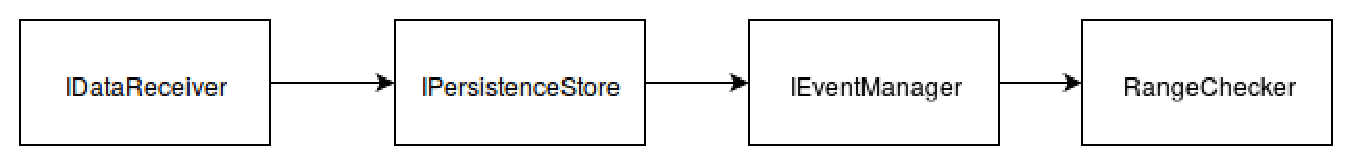
\includegraphics[width=\textwidth]{Figures/LogicArchitecture/Server/FlowDiagramNewRange}
\caption{Server, Flusso Dati Nuovo Range}
\end{figure}

\newpage

Prima di passare alla struttura \`e secondo noi utile andare a definire l'interazione del configurator in quanto \`e l'unica entit\`a attiva che non si basa effettivamente sui flussi e che contiene l'entry point di tutto il server.

\begin{figure}[h]
\centering
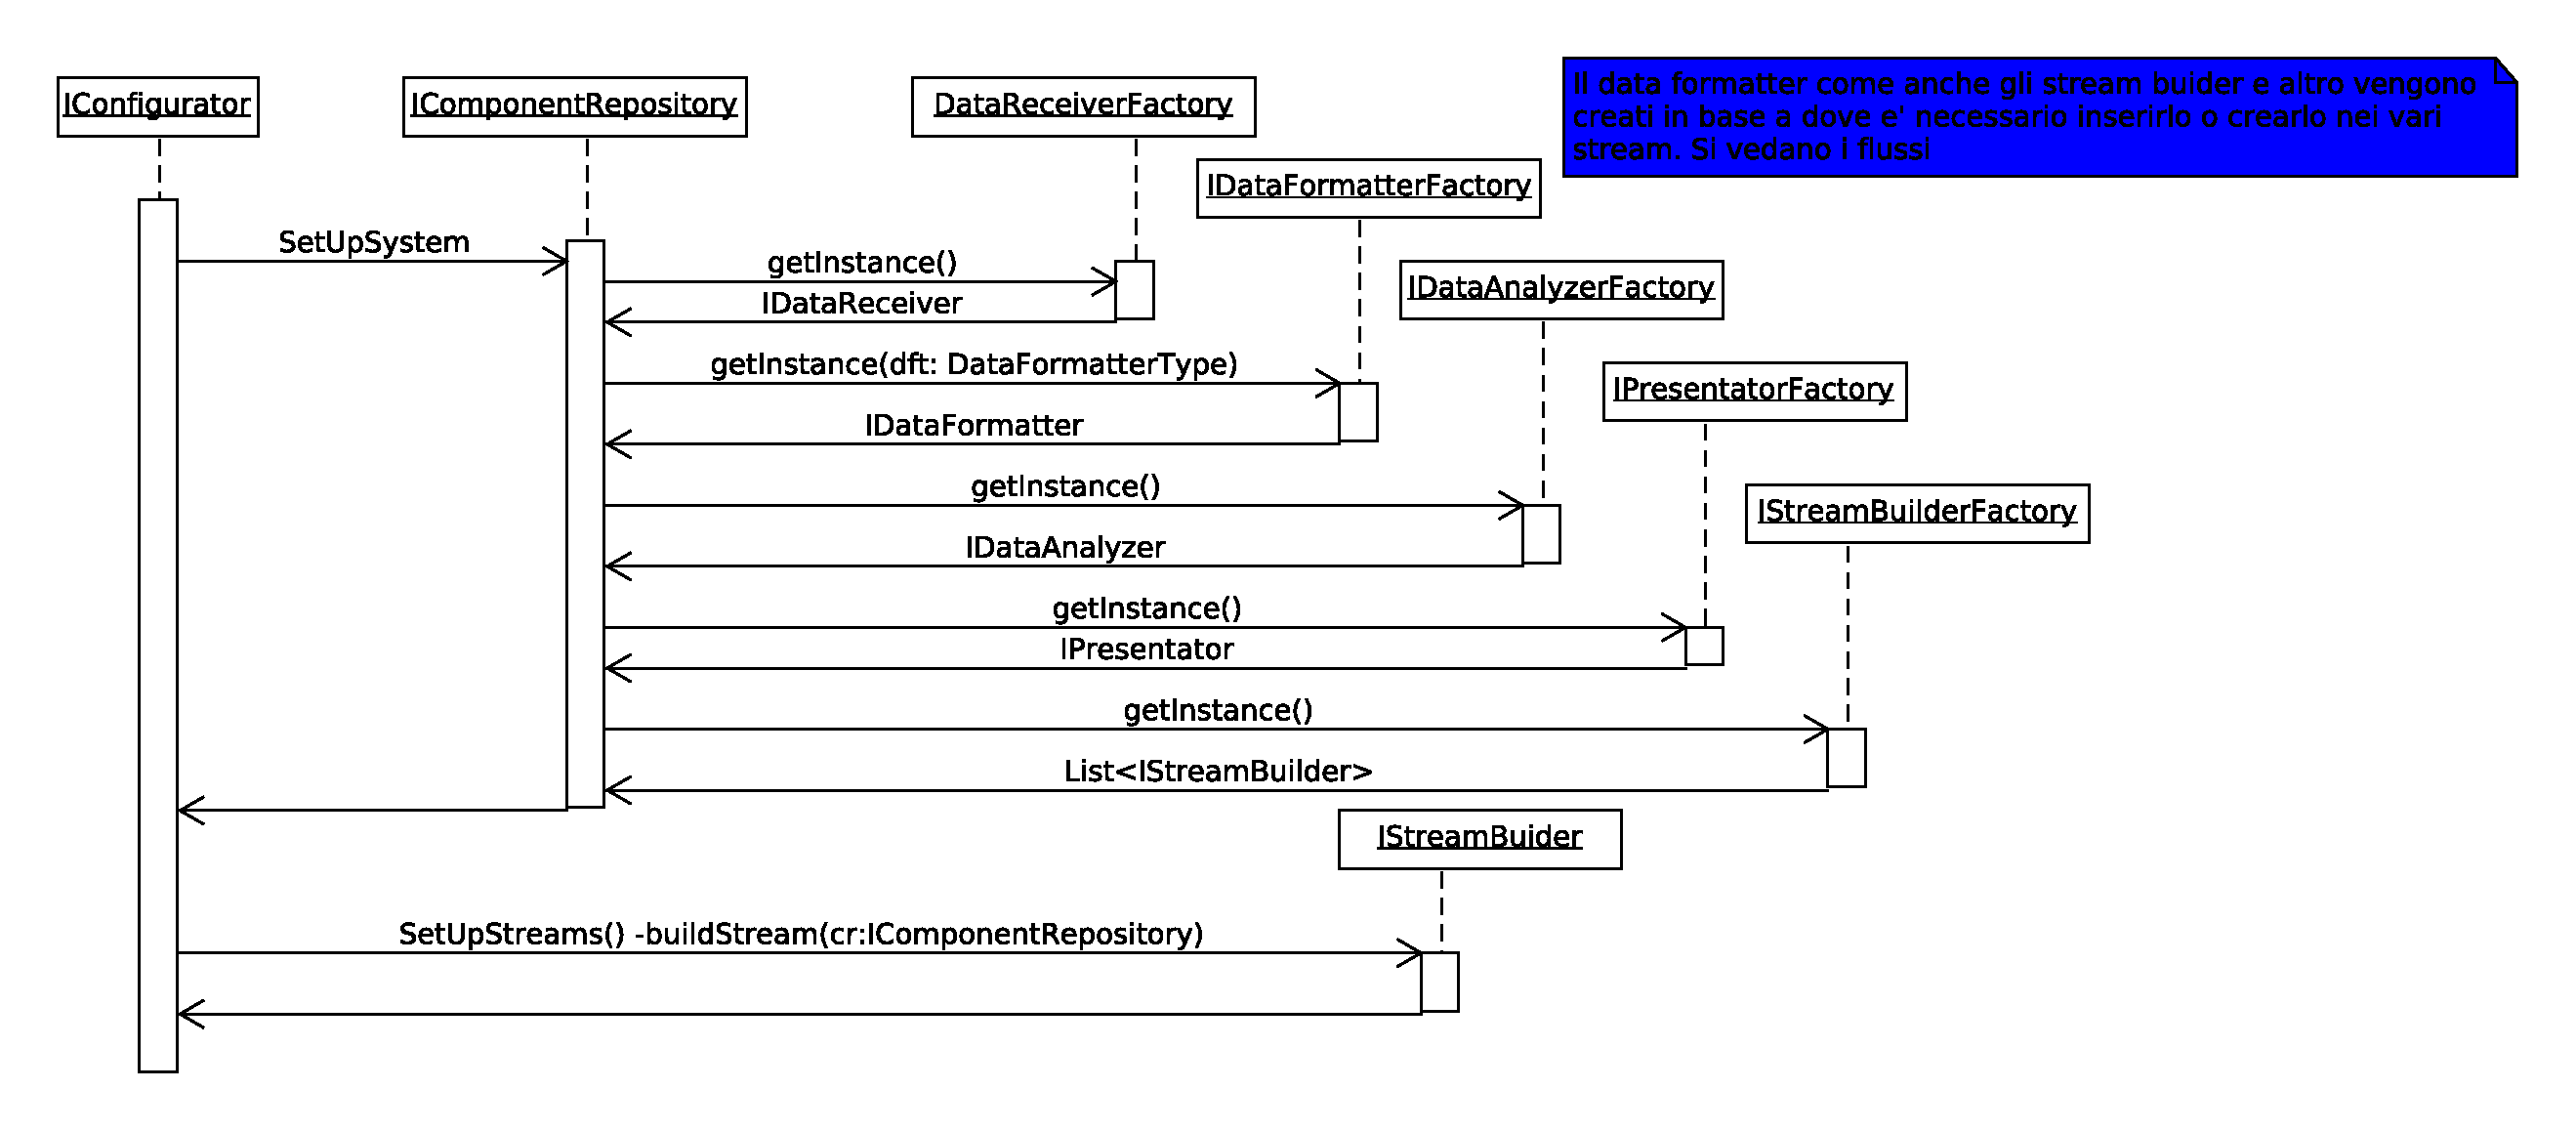
\includegraphics[width=\textwidth]{Figures/LogicArchitecture/Server/IConfiguratorInteraction}
\caption{Server, IConfigurator Interaction}
\end{figure}

\newpage

\begin{center}
\textbf{Struttura}
\end{center}

Nella struttura dell'analisi del problema abbiamo varie differenze, anche a livello di interfaccia, dovute al cambio di paradigma o ad altre motivazioni, di seguito verranno elencate per rendendere tutto pi\`u chiaro:

\begin{itemize}
\item IDataReceiver: non esiste pi\`u il metodo \textit{Receive} perch\'e non si ipotizza pi\`u un'approccio a polling e quindi non \`e necessaria questa funzionalit\`a, mentre invece viene esposto un metodo che da la possibilit\`a di ottenere lo stream di dati associato all'arrivo di un nuovo valore dall'esterno.
\item Tutto ci\`o che in precedenza, nel diagramma dell'interazione, era modellato attraverso una chiamata a procedura e veniva effettuata all'arrivo di un nuovo dato, ora viene convertito in funzioni che prendono in ingresso un dato stream e lo modificano restituendo un nuovo stream all'inizio del sistema in modo che, in questa fase, si \`e in grado di costruire e comporre i vari flussi che poi verranno elaborati attraverso l'infrastruttura.
\item Per separare ancora di pi\`u i vari flussi di stream indicati precedentemente e per separare i compiti di creazione dei vari stream si sono ideate delle classi \textit{factories} che assembleranno i vari componenti a tale scopo.
\item Sono stati impostati come oggetti sigleton i componenti \textit{EventManager e PersistenceStore}
\item \`E stato ampliato la parte del persistenceStore in modo da differenziare i vari compiti di salvataggio e caricamento attraverso diversi oggetti.
\item Il DataReceiver \`e stato differenziato tra dati provenienti dai sensori e dati provenienti dall'utente, come le richieste di un nuovo range o la richiesta di dati. Questo ha di fatto portato all'eliminazione dell'oggetto presentator individuato precedentemente.
\end{itemize}

\begin{sidewaysfigure}[h]
\centering
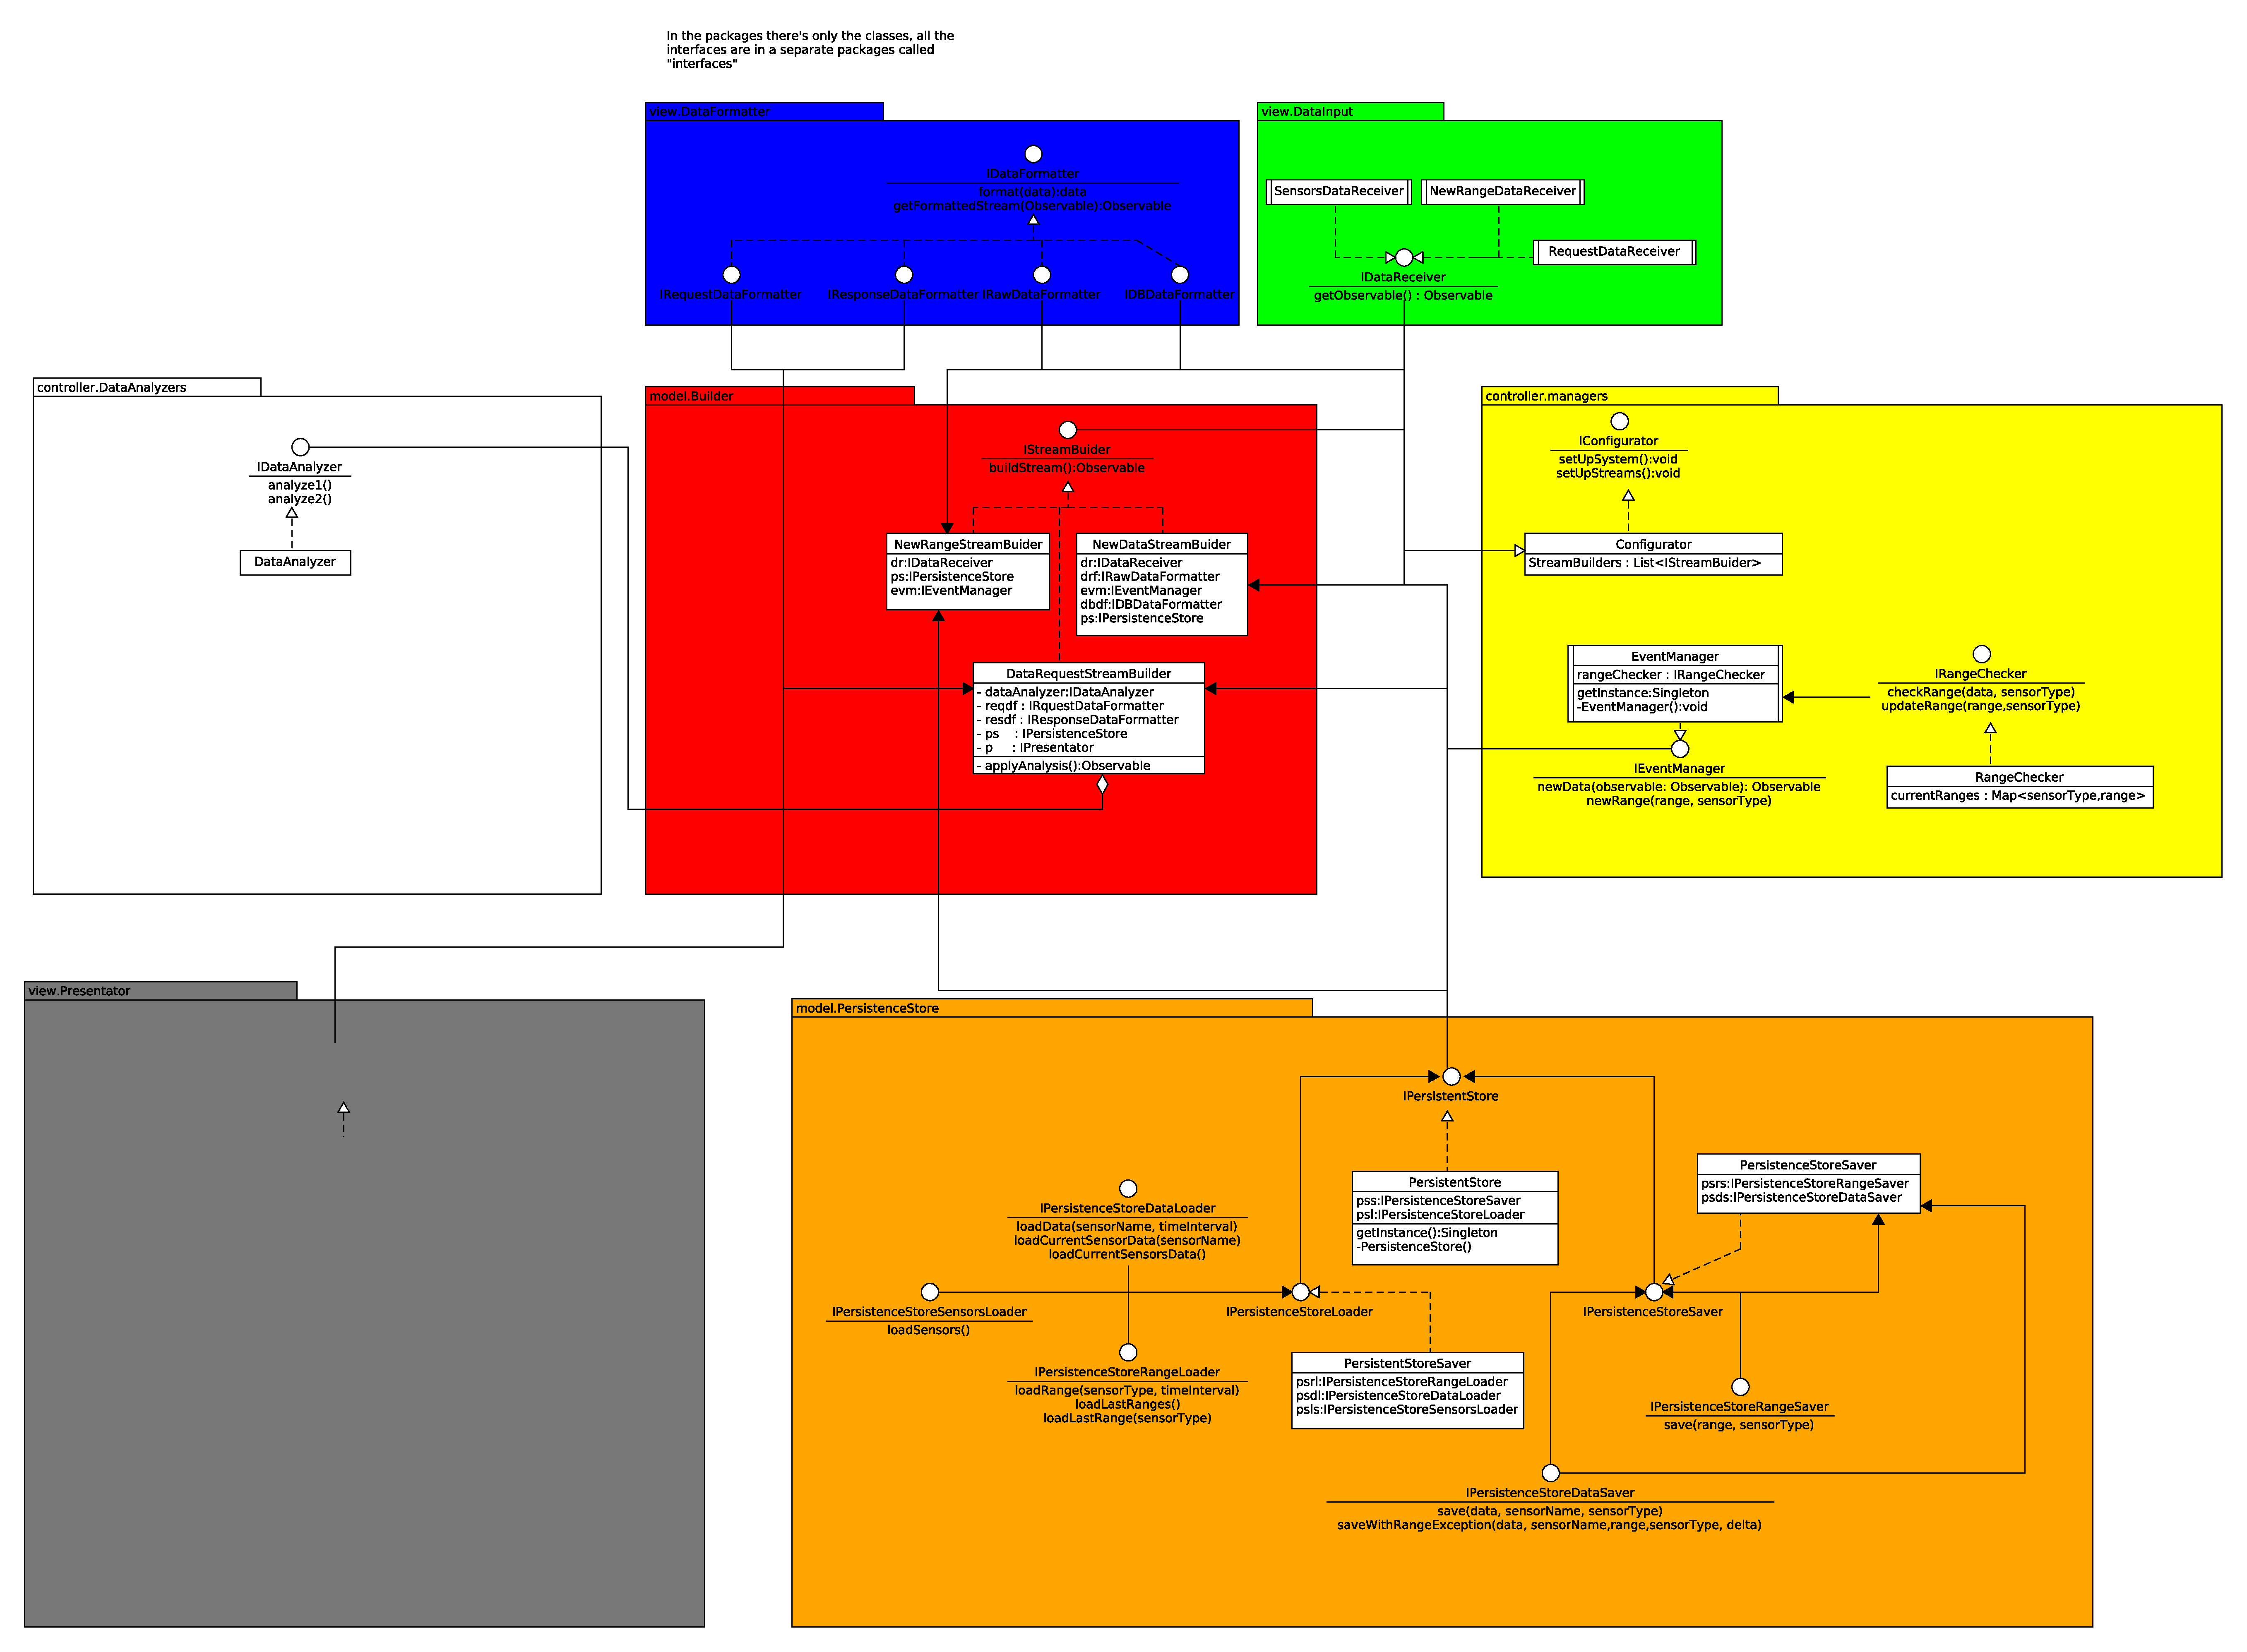
\includegraphics[width=\textwidth]{Figures/LogicArchitecture/Server/Structure}
\caption{Server, Struttura Architettura Logica}
\end{sidewaysfigure}

\afterpage{\clearpage}

\newpage

\begin{center}
\textbf{Comportamento}
\end{center}

Per quanto riguarda il comportamento delle varie parti del sistema verranno illustrate quelle principali e descritti gli stati principali incui questi componenti verranno a trovarsi. In particolare verranno omessi tutti quei componenti che effettivamente si occupano solamente della trasformazione degli stream in quanto non posseggono effettivamente uno stato, ma consistono in degli algoritmi che, dato un flusso in ingresso, gli applicano delle apposite trasformazioni e restituiscono un flusso in uscita.

\begin{figure}[h]
\centering
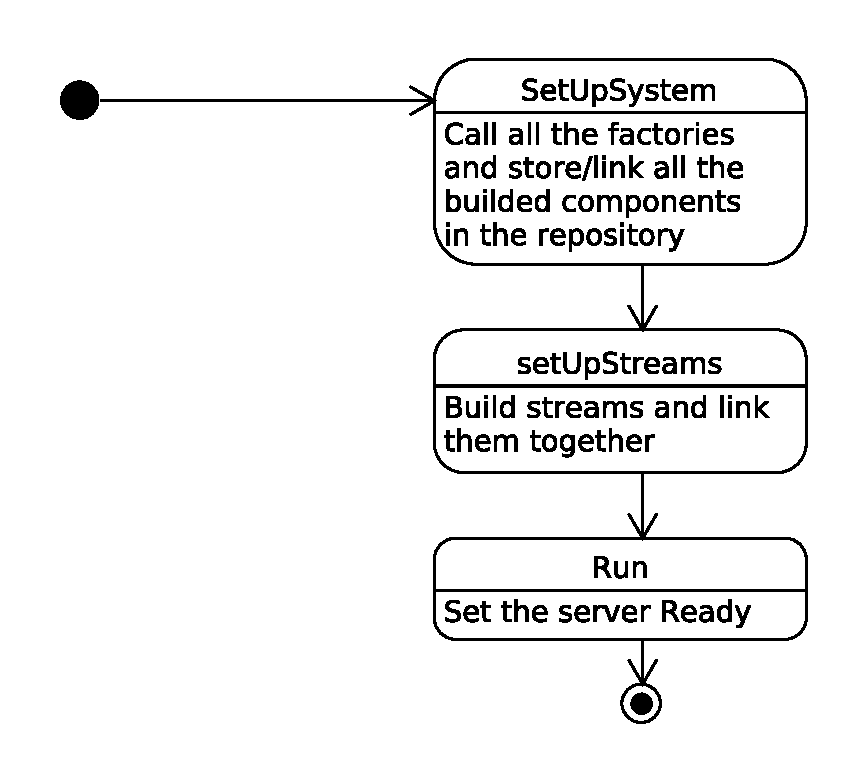
\includegraphics[scale=0.5]{Figures/LogicArchitecture/Server/IConfiguratorBehavior}
\caption{Server, IConfigurator Behavior}
\end{figure}

Come si pu\`o vedere dalla figura sovrastante il componente IConfigurator sar\`a quello che si occuper\`a di attivare tutto il sistema server occupandosi di rendere tutto operativo e pronto per le richieste da soddisfare. Questo avviene appunto in fasi, incui prima viene settato il tutto attraverso una fase di creazione di tutti i componenti necessari, poi avviene la creazione dei flussi che si occuperanno del flow dei dati ed infine si attiveranno questi flussi in modo che siano attivi.

\begin{figure}[h]
\centering
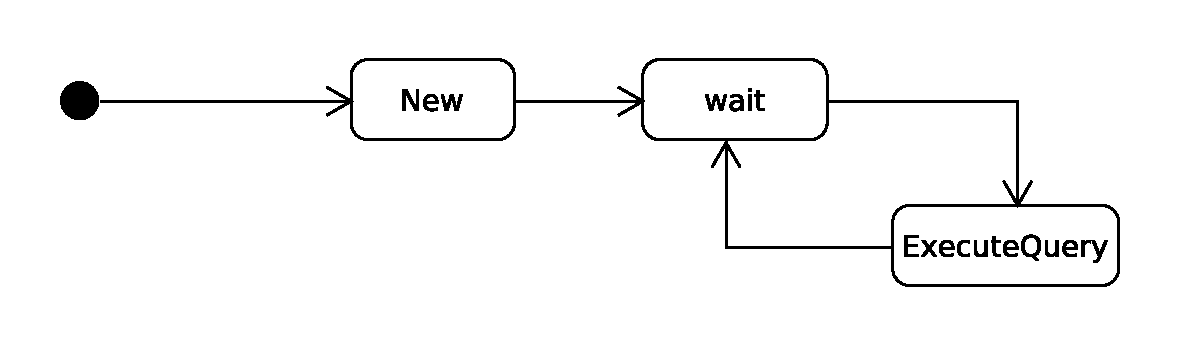
\includegraphics[width=\textwidth]{Figures/LogicArchitecture/Server/IPersistenceStoreBehavior}
\caption{Server, IPersistenceStore Behavior}
\end{figure}

Il comportamento del persistence store rimane molto semplice: una volta creato, attende la richiesta da parte del sistema per la memorizzazione dei dati.
Quando una richiesta avviene allora si attiva una delle parti che si occupano di leggere o scrivere all'interno del persistence store e effettuano l'operazione, per poi tornare in attesa di ulteriori operazioni. Si aggiunge inoltre che questo componente come l'eventManager sono componenti singleton, e quindi \`e presente solamente un'istanza di questo in tutto il sistema.

\begin{figure}[h]
\centering
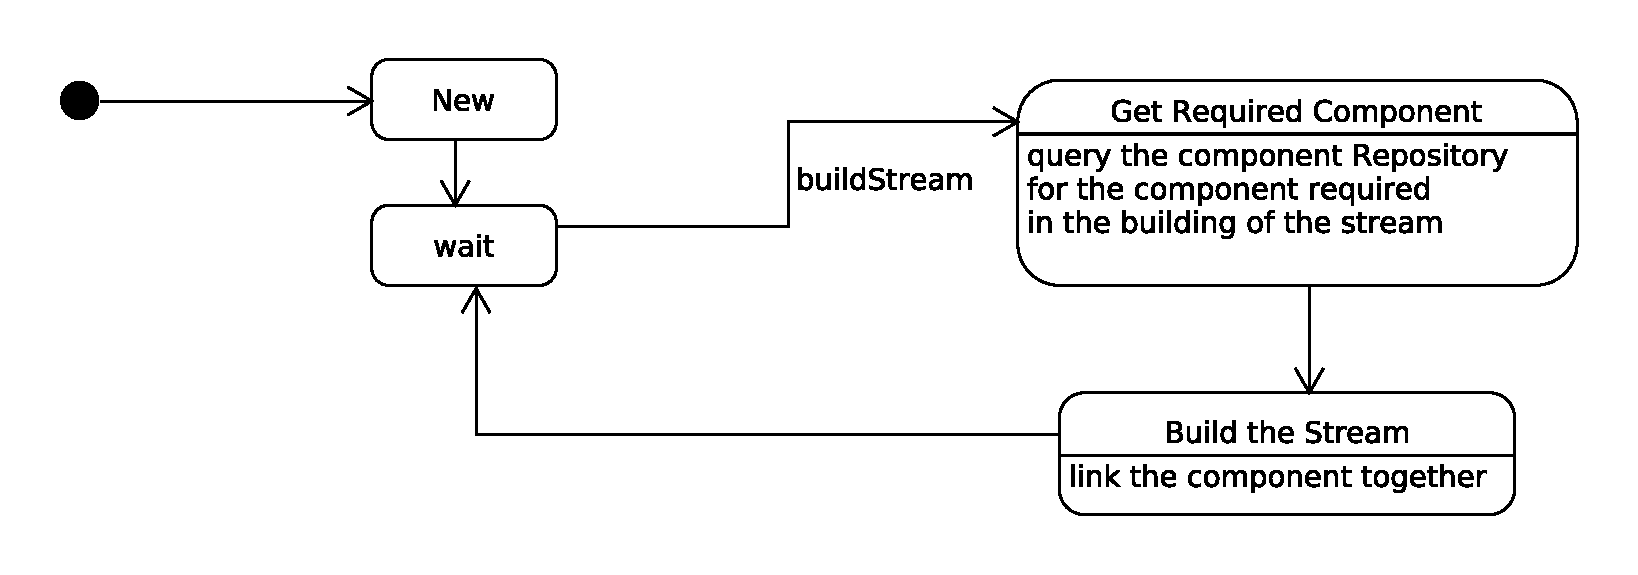
\includegraphics[width=\textwidth]{Figures/LogicArchitecture/Server/IStreamBuiderBehavior}
\caption{Server, IStreamBuilder Behavior}
\end{figure}

Lo stream builder anch'esso risulta molto semplice perch\'e viene chiamato da altri componenti, nel suo caso dal configurator stesso, e per questo presenta due stati come il caso precedente, \textit{New e Wait}. All'arrivo di una richiesta il componente richiede i vari blocchi necessari per la costruzione dello stream direttamente dal componentRepository e, una volta ottenuti li collega assieme per costruire il flusso che poi restituir\`a al configurator stesso.

\subsection{Gap di Astrazione}

In questa sezione aggiungeremo tutti i tipi di astrazioni richiesti per affrontare il progetto e che non sono direttamente fruibili attraverso la tecnologia di riferimento.

\begin{enumerate}
  \item Web Server: Data la necessit\`a di comunicare attraverso la rete \`e necessario che si utilizzi un paradigma a message-passing o attraverso chiamate asincrone, soprattutto per la comunicazione che avviene tra il raspberry e il server.
  \item Continuous Integration, Testing and collaborative source control: Lavorando in gruppo sullo stesso repository \`e necessario impostare il lavoro affinch\'e sia possibile effettuare modifiche in maniera indipendente gli uni dagli altri e allo stesso modo sia possibile controllare automaticamente che i test predisposti e le modifiche effettuate siano coerenti con le specifiche e che il building del progetto sia in ogni caso garantito.
  \item{Paradigmi Eterogenei}: si \`e deciso di utilizzare dei paradigmi diversi dal OOP classico e questo pu\`o portare a problematiche di utilizzo per via dell'inesperienza. Tuttavia queste non vengono fornite direttamente dal linguaggio e quindi si necessitano soluzioni al problema.
\end{enumerate}

\subsection{Analisi dei Rischi}

In questa sezione verranno elencati i rischi che si potranno incontrare in un progetto di questo tipo fonrmalizzandoli fin da subito, prima di eseguire l'effettiva realizzazione dello stesso, in modo da poterli affontare e discutere preventivamente per essere pronti nel caso questi si verifichino.

\begin{itemize}
  \item Aumento dei Costi: \`e necessario porre particolare attenzione alla struttura hardware del sistema e di come i singoli componenti vanno ad interconnettersi assieme per evitare che si debbano affrontare dei costi aggiuntivi, a progetto gi\`a avviato, causati da una qualche mancanza o per via di un'estensione del progetto in corso d'opera.
  \item Quantitativo della memoria: l'adozione di un database NoSQL porta con se un certo livello di ridondanza e quindi questo pu\`o portare ad un aumento di utilizzo della memoria e di spazio. Il tutto va valutato accuratamente durante il progetto, magari attraverso una serie di prove in base a come \`e stutturato il dato inizialmente. Se il rischio quindi \`e reale e quanto \`e critico.
  \item Integrazione tra le tecnologie: un possibile rischio riguarda la difficolt\`a nell'integrare tutte le tecnologie che devono essere sfruttate nel progetto per riuscire a colmare l'abstraction gap e quindi riuscire a completare il progetto attraverso l'analisi appena completata.
\end{itemize}
